\section{Plan de actividades}

La creación de software se enfocó en la división de tareas desde el principio y la creación de una estructura que sustentaría todo el proyecto. Primero y principalmente creamos una ilustración que explicaba graficamente la forma en que sería el proyecto. Con el tiempo, esta ilustración se modificó en función de las tareas que surgían y las habilidades de cada miembro del equipo o su desempeño con respecto a las propuestas. 

La metodologia que se utilizo fue mediante una comunicacion activa para aclarar la planificacion de los objetivos y analizar en cada encuentro la realizacion de dichas actividades, donde se acordó que uno de los objetivos principales para llevar a cabo era el diseño que iba a presentar la pagina, para luego poder desarrollar la parte funcional y programar un entorno de desarrollo utilizando tecnologias para el backend. Después de haber cumplido con la importante tarea de haber trabajado en el Backend y en el Frontend quedaba poner a prueba y asegurar que tuviera un funcionamiento óptimo para la experiencia del usuario, ya que la pagina debía cumplir con las funciones recientemente hechas y, por otro lado, la interfaz del usuario debía ser intuitiva y fácil de usar para así poder corregir y ajustar los errores que se presentaban.

Las herramientas que tuvimos a nuestro favor y para llevar a cabo el plan de actividades fue el gestor de proyectos \href{https://trello.com/b/gpuunRxX/tp-ids}{Trello}, donde pudimos listar las tareas entre los integrantes y asi tener un seguimiento de cada una. El desarrollo de la pagina lo logramos hacer gracias a la implementación de Git y \href{https://github.com/MaxiFttInst/UBA_TP_IDS}{GitHub}, y otros programas como Visual Studio Code, MySQLite, Docker, entre otros.

Los integrantes del proyecto contaron con una división de roles y responsabilidades que tuvieron que cumplir como Desarrolladores de Backend y Frontend, pero mas allá del rol principalmente impuesto se cada uno logró contribuir en cualquiera de las áreas, para ello realizábamos encuentros para charlar las cuestiones que se nos dificultaba, trabajar como equipo y documentar cualquier cambio que hiciéramos por medio de un grupo de Discord.

\subsection{Creación de frontend}

El desarrollo del Frontend fue una de las primeras tareas a realizar, ya que antes de comenzar la codificación se presentó un diseño y planificación de la estructura con la implementación de \textbf{HTML}, para la base de la página web, \textbf{CSS}, para definir el aspecto visual y aplicar estilos, y \textbf{JavaScript}, para agregar una interactividad y dinamismo.


\subsubsection{calendario}

La implementación de un calendario es importante a la hora de realizar las reservas, por que es la conexión entre el cliente y la funcionalidad, por lo que se tuvo que implementar desarrollo en el Front para la vista, como en el Back para la funcionalidad.


\subsection{Crear base de datos}


La base de datos es una parte crucial del trabajo ya que almacena toda la informacion de la pagina, ya sean las reservas, habitaciones e imagenes. Por lo que se implemento distintos diseños para realizar dicha base de datos como se pueden observar en las figuras \ref{fig:BD1} y \ref{fig:BD2}



\begin{figure}
    \centering
    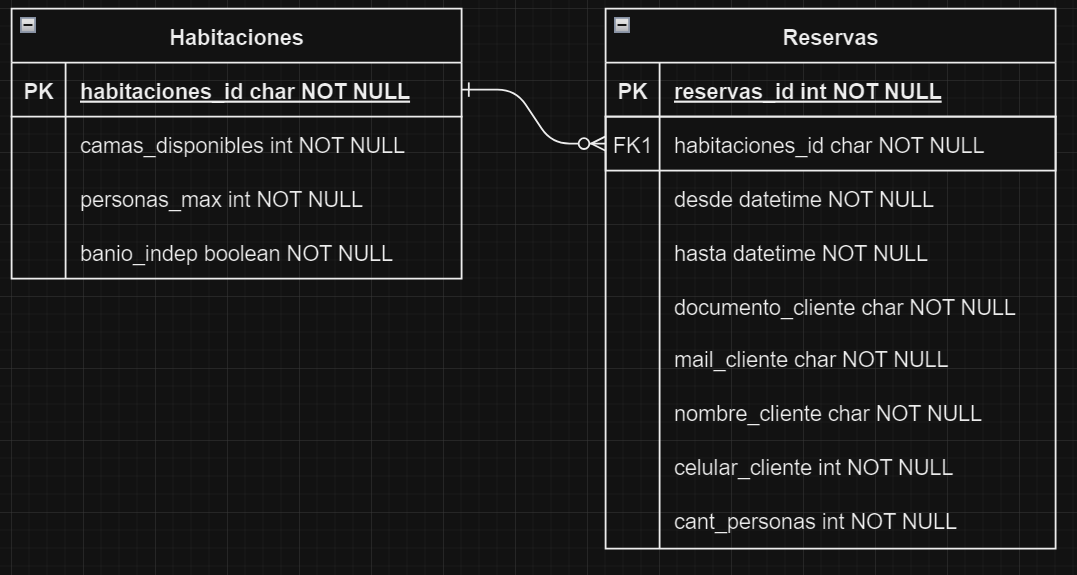
\includegraphics[width=0.75\linewidth]{images/base de datos 1.png}
    \caption{Idea principal de la Base de Datos}
    \label{fig:BD1}
\end{figure}


\begin{figure}
    \centering
    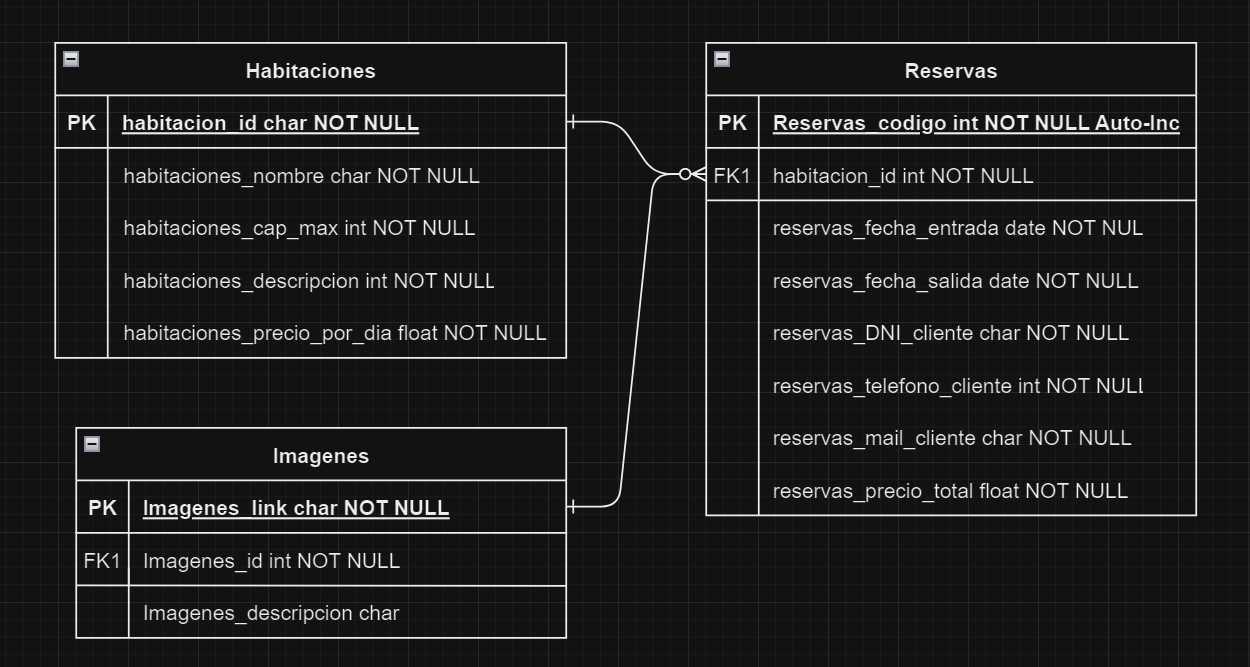
\includegraphics[width=0.75\linewidth]{images/base de datos final.png}
    \caption{Idea final de la Base de Datos}
    \label{fig:BD2}
\end{figure}


\subsection{Realizacion de requests}

El realizar los requests era necesario para todas las tablas de la base de datos del proyecto, ya sea para obtener los datos de las cabañas, como realizar la reserva o agregar alguna imagen de la cabaña, es por eso que se llevaron a cabo diferentes tareas donde se vieron implementadas cada una de estas funciones del CRUD (Create, Read, Update, Delete) para las diferentes tablas

\subsubsection{GET}

Los requests del tipo GET se utilizan para obtener datos del servidor, es por eso que se utilizó para saber que cabañas hay con disponibilidad, las reservas que hizo el mismo cliente o mismo para ver las imagenes implementadas.

\subsubsection{POST}

Los requests del tipo POST se utilizan para enviar datos al servidor, su implementación fue necesaria y esencial para realizar las mismas reservas y así poder guardarlas en la base de datos.

\subsubsection{PATCH}

El PATCH se utiliza para poder actualizar dichos datos del servidor, y fue necesario en el caso que se quiera modificar algún dato o el mismo día que se haya realizado la reserva.

\subsubsection{DELETE}

Los requests del tipo DELETE son utilizados para eliminar algún dato del servidor, para ello es de importancia su uso en el caso que se quiera cancelar una reserva a nombre de un cliente.

\subsection{Creación de backend (API)}

La Interfaz de Programación de Aplicaciones es esencial para el Backend ya que es el gestor de lógica del servidor, sus operación junto a la base de datos y su comunicación con el Front. Su creación era necesaria para la conexión con la Base de Datos, las rutas, el propio servidor y los mismos Endpoints de la API en el cual estaban presentes todas las operaciones del CRUD.


\subsection{Cargado de imágenes en el drive}


Las imágenes son necesarias para poder generar una mejor experiencia con el usuario, ya que se muestran algunas de las cabañas en cuestión o mismo las instalaciones, actividades o servicio. Es por eso que se implementó el uso de \href{https://drive.google.com/drive/folders/1rzJS4rG295Mjmsm-0Xie7m3Bs8-YsvL0}{Google Drive} para cargar las imágenes, donde están todas subidas en una carpeta de llamada "Imágenes". Su implementación es necesaria por la buena gestión de archivos.


\subsection{Backoffice}

El Backoffice es una tarea que se precisaba para que el administrador sea capaz de modificar la pagina en el caso que sugiera algún cambio, ya sea en las imágenes, como en las reservas o las mismas cabañas. El administrador debe ser capaz de poder gestionar la información del mismo cliente en el caso que se precise para las reservas realizadas, o también debe tener la posibilidad de administrar la información de las mismas cabañas de la pagina, ya sea para implementar o quitar información. El administrador debe tener la posibilidad de modificar y gestionar la pagina de la posada con operaciones del CRUD de una forma sencilla.

\subsection{Hosteo de la base de datos y la página en pythonanywhere.}

Para exhibir la pagina de la posada se utilizó Pythonanywhere, el cual nos permite tener una conexion entre los datos almacenados y la misma pagina.
